\section{1. May 2021 - Report (a summary)}
In order to investigate the edge-length ratio, the first approach was to draw simple example graphs and simply look for the edge-length ratio behaviour.
\subsection{First example - One triangle}
\begin{lemma}
	There exists a graph which is not drawable on a fixed grid with an edge-length ratio of 1.
\end{lemma}
\begin{proof}
	Consider a triangle. In order to draw it with equally long edge lengths $l$, the height must value $\frac{\sqrt{3}}{2}l$.
		\begin{figure}[H]
		\centering
		\includegraphics[page=1]{drawings/previous-results.pdf}
		\caption{Triangle}
	\end{figure}
	Since $\sqrt{3}$ is an irrational number, therefore there exists no combination of coordinates on a grid in order to represent the triangle. Otherwise, there would exists two integers to represent $\sqrt{3}$ as a fraction. Therefore, there exists no drawing of a triangle with edge-length ratio 1.
\end{proof}
If we want to get close to an egde-length ratio of 1, we are bound to approximate the cofactor $\sqrt{3}/2$ in the height of the triangle. 
\begin{observation}
	W.l.o.g., let the given grid be of size $g \times g, g \in \N$. For $c$, it holds:
	\begin{align*}
		c = 0,8660254 \approx \frac{\sqrt{3}}{2}
	\end{align*}
 	Then, it is better for the edge-length ratio to draw the triangle as large as possible on the grid so that the approximation gets more precise.
\end{observation}
So one first intuition is to use all the given area on the grid. 
\begin{figure}[H]
	\centering
	\begin{subfigure}{0.4\textwidth}
		\centering
		\includegraphics[page=2]{drawings/previous-results.pdf}
		\caption*{Triangle A}
	\end{subfigure}
	\begin{subfigure}{0.4\textwidth}
	\centering
	\includegraphics[page=3]{drawings/previous-results.pdf}
	\caption*{Triangle B}
\end{subfigure}
\end{figure}
\begin{align*}
	\text{ratio}_A < \text{ratio}_B
\end{align*}
\subsection{Second example - $m$ Triangles, nested and triconnected}
Take a look at the following drawing:
\begin{figure}[H]
	\centering
	\begin{subfigure}{0.8\textwidth}
		\centering
		\includegraphics[page=4]{drawings/previous-results.pdf}
		\caption*{Drawing $\Gamma$ of $m$ nested triangles}
	\end{subfigure}
\end{figure}
The $i$-th triangle is defined as the connected set of vertices $\{a_i,b_i,c_i\}$. One difficulty of a resizing is the nestedness of the triangles. On one hand, if an inner triangle gets larger, then the whole drawing might get larger, meaning that the longest edge got longer. On the other hand, if the triangles distances differ by a constant, the diagonal, orange-colored edge stay small.\\
\begin{observation}The solution is to reposition the vertices of every triangle. One can imagine, that each inner triangle is \grqq flipped\grqq~by one more turn. No bends were used yet.
\end{observation}
Then, the following new drawing is derived by this approach. 
\begin{figure}[H]
	\centering
	\begin{subfigure}{0.8\textwidth}
		\centering
		\includegraphics[page=5]{drawings/previous-results.pdf}
		\caption*{New drawing $\Gamma'$ of $m$ nested triangles}
	\end{subfigure}
\end{figure}
With help of this vertex repositioning, the shortest edge now is a longer one - still illustrated in orange. When the shortest and the longest edge are within one of the $m$ triangles and the distance between each triangle is constant, then the ratio lies in $\mathcal{O}(n)$ and is independent of the grid size.
\subsection{Variant of the second example - more edges!}
The previous example has got more edges in a way, that each vertex is of degree at least 4. The following drawing illustrates the altered graph:
\begin{figure}[H]
	\centering
	\begin{subfigure}{0.8\textwidth}
		\centering
		\includegraphics[page=6]{drawings/previous-results.pdf}
		\caption*{Drawing of altered previous graph, new edges are illustrated with a green color}
	\end{subfigure}
\end{figure}
Now, the \grqq turn\grqq~of the triangles is restricted since we might violate the property of planarity. One question was, how the triangles should be drawn generally. So, in order to get an idea, the drawing for $m=2$ was optimized until there is nothing left to do.
\begin{observation}
	By \grqq keeping the triangles close to each other\grqq, it is possible to further reduce the edge-length ratio.
\end{observation}
\begin{figure}[H]
	\centering
	\begin{subfigure}{0.8\textwidth}
		\centering
		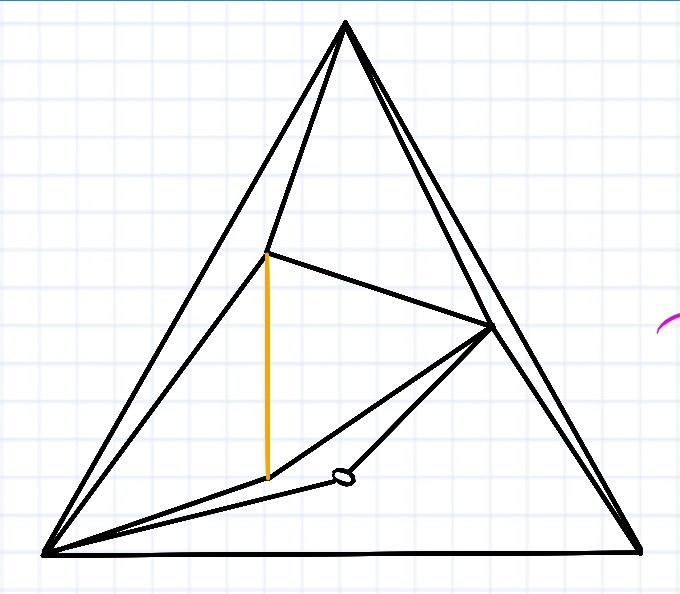
\includegraphics[width=0.5\linewidth]{drawings/two_triangles_1.jpg}
		\caption{Start the optimization here. The shortest edge is illustrated with an orange color}
	\end{subfigure}
	\begin{subfigure}{0.8\textwidth}
	\centering
	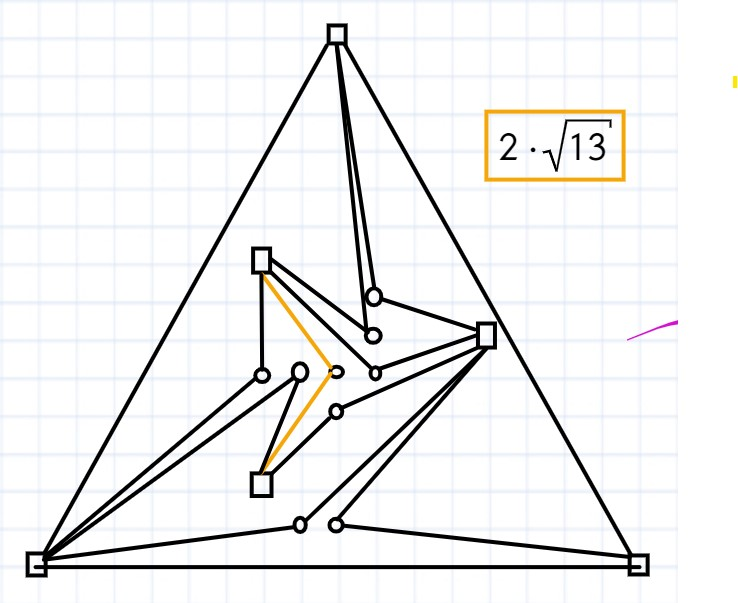
\includegraphics[width=0.5\linewidth]{drawings/two_triangles_2.jpg}
	\caption{Bends were included. The Unit Length equals the length of one box.}
\end{subfigure}
	\begin{subfigure}{0.8\textwidth}
	\centering
	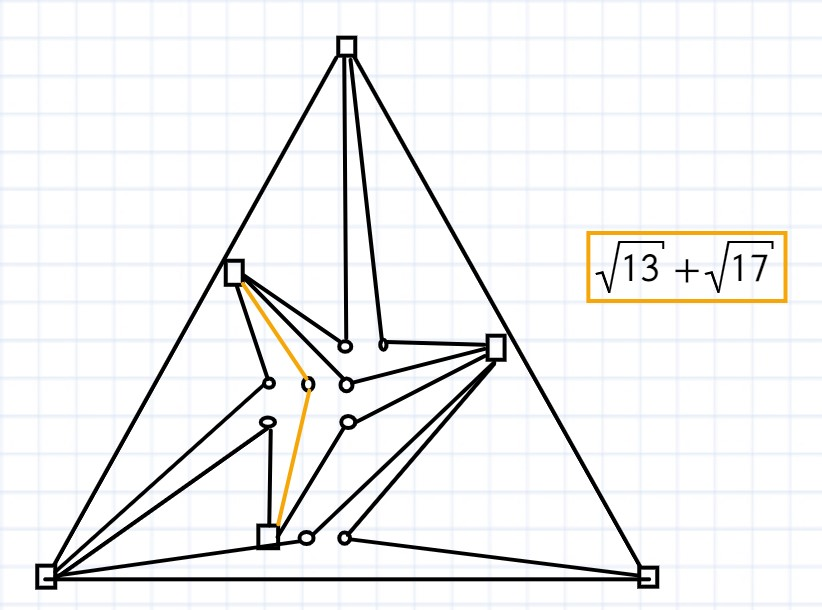
\includegraphics[width=0.5\linewidth]{drawings/two_triangles_3.jpg}
	\caption{Vertex and bend repositioned for a better result}
\end{subfigure}
	\begin{subfigure}{0.8\textwidth}
	\centering
	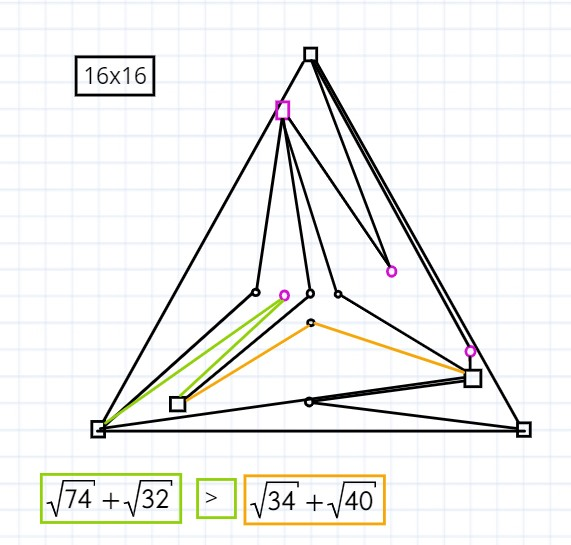
\includegraphics[width=0.5\linewidth]{drawings/two_triangles_4.jpg}
	\caption{After greedily elongate the shortest edge in a couple of iterations, it gets clear, how the triangles could be drawn with a satisfying ratio.}
\end{subfigure}
\end{figure}
This leads to the following approach, the discussion to the steps follow further below.
\begin{algorithm}[H]
	\KwIn{Graph consisting of $m$ triangles connected as illustrated above, Gridsize, one bend allowed}
	\KwOut{Drawing with a satisfying edge-length ratio}
	Draw the outermost triangle as big as possible on the grid with the approximated height\\
	\For{$i=2$ to $m$}{
		Place the $i$-th triangle inside the predecessor by a constant $c$\\
		Place bend points between those triangles and draw the edges with length bound by the shortest edge of the inner triangle and the longest edge of the outer triangle
	}
\caption{Algorithm sketch for a drawing of the example graph}
\end{algorithm}
Details:
\begin{enumerate}
	\item Recall the approximation for a uni-sized triangle of the first section for the triangle.
	\item It is important to have grid points between two consecutive triangle drawings. The bends must be placed somewhere.
	\item To get an idea, how exactly the bend points are set, please, take a look at the following picture.
	\begin{figure}[H]
		\centering
			\begin{subfigure}{0.8\textwidth}
			\centering
			\includegraphics[width=0.8\linewidth,page=7]{drawings/previous-results.pdf}
			\caption{This is the output of the algorithm with $m = 2$.}
		\end{subfigure}
		\begin{subfigure}{0.8\textwidth}
			\centering
			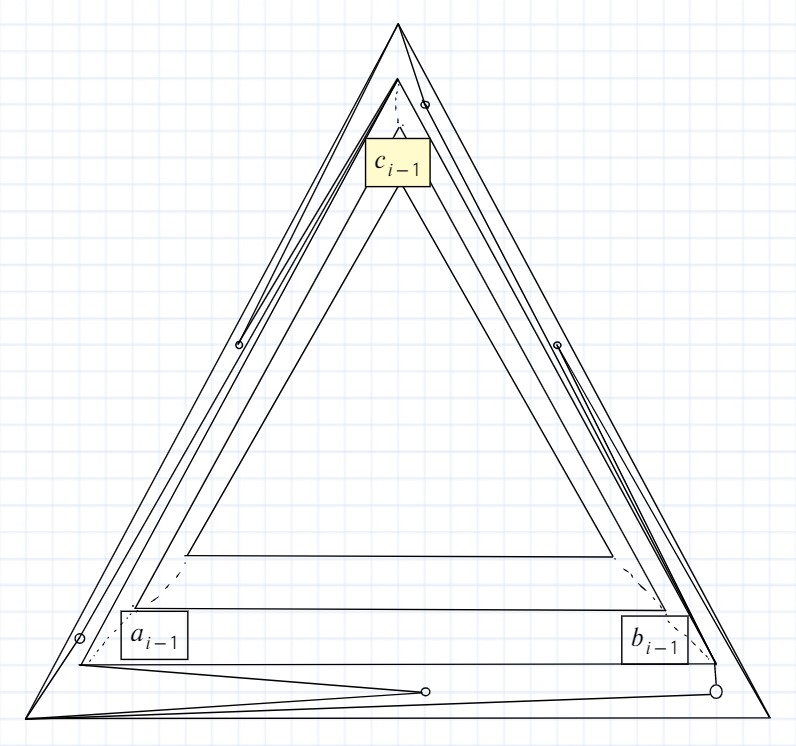
\includegraphics[width=0.8\linewidth]{drawings/variant_triangles_1.jpg}
			\caption{In this case, deg($a_1$)=5, deg($b_1$) = 3, deg($c_1$) = 4}
		\end{subfigure}

	\end{figure}
	The bend point for w.l.o.g. $(a_{i-1},a_i)$ lies centralized between $a_{i-1}, b_{i-1},a_i, b_i$. Analogue for the other ones. The bend point for w.l.o.g. $(a_{i-1},b_i$ lies below $b$. To guarantee the existence of those points, it is important not to choose the \grqq shrinking constant\grqq~$c$ too small.
\end{enumerate}
	\begin{lemma}
		With one bend allowed per edge, the graph above, inheriting $m$ triangles, will have an edge-length ratio in $\mathcal{O}(n)$.
	\end{lemma}
	\begin{proof}
		If the construction of the drawing is correct, then the innermost triangle $t_m$ will inherit the shortest edge and the outerface $t_1$ will contain the longest edge. Since the triangles have a constant distance pairwise, the differences between the edge lengths of the outermost and the innermost triangle is linear to the amount of triangles. Therefore, the ratio between the longest edge on the outermost triangle and the shortest edge on the innermost triangle grows linear with the amount of triangles. Hence, the ratio lies in $\mathcal{O}(n)$.
	\end{proof}
\subsection{Third example - a complete binary tree with depth $d$}
A binary tree is 1-connected. It is of interest, how the edge-length ratio behaves for a given depth $d$. In order to get a feeling, drawings of uniform long edges were created and it was observed, at which depth it is not possible to place further vertices.
\begin{observation}
	When the drawing starts with horizontal or vertical edges, it is not possible to draw a complete binary tree of depth $5$ with an edge-length ratio of 1.
\end{observation}
	\begin{figure}[H]
		\centering
		\begin{subfigure}{0.8\textwidth}
			\centering
			\includegraphics[width=0.5\linewidth,page=9]{drawings/Erste-Beispiele.pdf}
			\caption*{At some point, there is simply not enough area for $2^d$ vertices}
		\end{subfigure}
	\end{figure}
\begin{observation}
	If starting diagonally first, a complete binary tree of depth 5 is drawable on a 11x11 grid with a ratio of $\sqrt{2}$.
\end{observation}
	\begin{figure}[H]
	\centering
	\begin{subfigure}{0.8\textwidth}
		\centering
		\includegraphics[width=0.5\linewidth,page=9]{drawings/bintree-without-bends.jpg}
		\caption*{It seems that, when starting diagonally, there might be more grid points availiable}
	\end{subfigure}
\end{figure}
\begin{lemma}
	Allowing one bend, it is possible to draw a complete binary tree of depth $5$ with an edge-length ratio of 1.
\end{lemma}
\begin{proof}
		\begin{figure}[H]
		\centering
		\begin{subfigure}{0.8\textwidth}
			\centering
			\includegraphics[width=0.5\linewidth,page=9]{drawings/bintree-with-bends.jpg}
			\caption*{Using bends, all edges are of the same length}
		\end{subfigure}
	\end{figure}
\end{proof}
\begin{theorem}
	A complete binary tree with depth $d$ can be drawn with an edge-length ratio of $\mathcal{O}(\sqrt{n})$
\end{theorem}
\begin{proof}[Sketch of a proof]
	As already seen, for the depth up to 5, the edge-length ratio values 1. Incrementally, the drawing of $i$-th depth is achieved by copying the drawing of $i-1$ and each roots of the subtrees with a vertex. When looking at the drawing of depth $7$, then we observe that the ratio is the same as of the drawing with depth 6.
			\begin{figure}[H]
		\centering
		\begin{subfigure}{0.8\textwidth}
			\centering
			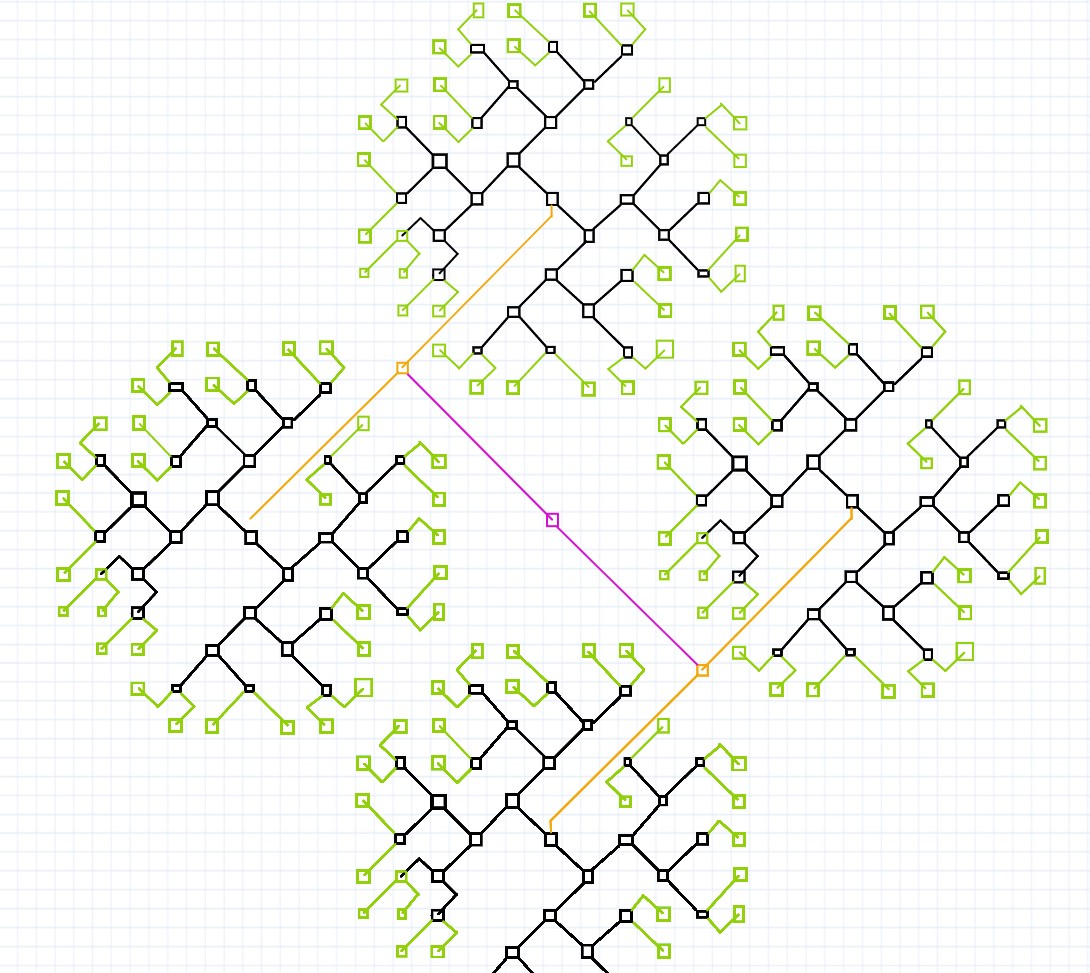
\includegraphics[width=\linewidth]{drawings/bintree-with-bends-depth-7.jpg}
			\caption*{Depth 6 in orange, depth 7 in purple}
		\end{subfigure}
	\end{figure}
	The ratio can be expressed as:
	\begin{align*}
		\text{ratio}_d = 2^{\lfloor\frac{d}{2}\rfloor-1} + \frac{1}{2}\in \mathcal{O}(n)
	\end{align*}
\end{proof}
\subsection{General observations / thoughts}
\begin{itemize}
	\item Draw large, thinking of one triangle
	\item \grqq twist\grqq a subgraph / component
	\item When components are nested, try to maintain a constant spacing
	\item Bend placement: either next to a vertex or in the center of a set of vertices
	\item Drawing diagonally is not a bad idea? (Binary tree)
	\item ???
\end{itemize}
